\chapter{Methods}
\label{chp:methods}
% ------------------------------------------------------------------------------

% CHAPTER INTRODUCTION
% * what is discussed in this chapter?
% * emulation is discussed, with focus in hydrology
% * introduce the tools needed for emulation: they will be explained later
%   in detail
% * simulation is used to explore
% * experiment: we mean here numerical experiment -> say it!

% ==============================================================================
\section{Hydrodynamical simulator}
% ==============================================================================
% * transfer functions
% * PDEs
% * https://en.wikipedia.org/wiki/Routing_(hydrology)
% * go for hydrodynamic simulation => more detailed, more complex, slower
% * (Hydrological models could even be considered "emulators" of the more
%   detailed PDE-simulators)

% ------------------------------------------------------------------------------
\subsection{FullSWOF\_2D-v1.07.00}
% ------------------------------------------------------------------------------
% * show the results of a simulation (cross-reference with channel simulation)
% * 

The numerical simulator which has been emulated in the two case studies presented in Chapter 3 is \citetalias{delestre_fullswof:_2017}. FullSWOF (Full Shallow Water equations for Overland Flow) is an \emph{open source} software solving the Shallow Water equations (SWE) over regular uniform grid using finite volumes method (FVM) %and numerical methods especially chosen for hydrodynamic purposes 
\autocite{the_fullswof_team_fullswof_2018}. \\
 
Water can enter the simulation domain through the boundaries (\emph{imposed discharge}) or with the rain.
Input discharge is fixed in space and time. Rainfall is applied uniformly to the simulation domain, but it is allowed to vary in time. If the option rain is activated, a \emph{rainfall file} with the rain hyetograph (the rainfall intensity as a function of time) has to be provided.   

SAY SOMETHING ABOUT INFILTRATION METHOD, ET NOT IMPLEMENTED, HOW WATER CAN EXIT .. 

In order to run simulations, FullSWOF needs at least the following inputs:
 % numeri al posto di paragraph
\paragraph{Topography file} A text file specifying the topography of the gridded simulation domain. This is done specifying the coordinates (x and y) of each grid cell and the respective elevation (z) with an x-y-z format 

\paragraph{Simulation parameters file} A text file defining the values of the simulation parameters. This can be generated with the function \textit{params2file} of the fswof2d package (see Appendix A.1.
Simulation parameters include:

\begin{itemize}
\itemsep0em
  \item Number of cells (x and y directions)
  \item Simulation duration
  \item Number of intermediate states saved
  \item Domain length
  \item Domain width
  \item Boundary conditions specifications
  \item Various settings for the numerical schemes
  \item Different physical parameters (friction coefficient, initial soil saturation, soil thickness, soil hydraulic conductivity, maximal infiltration). These parameters are spatially distributed. A unique value for the whole domain can be used or a value for every cell can be defined by giving to the simulator a text file specifying all of the values.\\
\end{itemize}

\paragraph{Initial conditions file} A text file defining the initial conditions of the simulation. It specifies the \emph{water depth}, the \emph{flow velocity in x} and the \emph{flow velocity in y} for all cells of the domain. \\ % All of these can also be set to \num{0}.\\

FullSWOF simulations generate five different \emph{output files}.
% numeri al posto di paragraph 
\paragraph{Initial simulation state file} reports the initial state (at $t = \SI{0}{\s}$) of the simulation. 
This corresponds to the initial conditions file.
\paragraph{Final simulation state file} reports the state of the simulation (at $t = t_{max}$).
\paragraph{Simulation states file} stores the whole evolution of the simulation: it begins with the initial conditions and ends with the final state.How many intermediate results to saved is set by the user in the parameters file.
\paragraph{Water budget/balance file} records how much water has been lost through the boundaries, how much has infiltrated and how much is present in the simulation domain.
\paragraph{Parameters file copy}. Useful to know which parameters were set to generate a given output.

In order to generate these files, interaction functions were developed with the open source tool \textit{Octave 4.2.1} \autocite{octave_community_gnu_2018}. The interaction functions were grouped into the Octave package \textit{fswof2d} available at \url{https://bitbucket.org/binello7/fswof2d}. For more information, refers to  Appendix A.1

% ------------------------------------------------------------------------------
% FULLSWOF2D PACKAGE
% * list the functions developed
% * high-level infos what functions do
%   - input
%   - output
%   - methods/operations
% * or move to appendix if no time
% * put just summary in main body:
%   "fswof2d has 18 functions with 20 methods to convert data, pre-processes
%    grids for efficient construction of simulation domain, interface Octave
%    engine (see Appendix X for details.)"

PUT IN APPENDIX A.1 
The package includes the following functions, all of which are distributed under \textit {GPLv3} license \autocite{smith_quick_2014}.
 
\begin{itemize}
\itemsep0em
  \item center2node.m
  \item csec\_channel2lvlsym.m
  \item dataconvert.m
  \item extrude\_csec.m
  \item huv2file.m
  \item matplotlib\_cm.m
  \item node2center.m
  \item params2file.m
  \item read\_params.m
  \item topo2file.m
\end{itemize}

% ==============================================================================
\section{Emulation}
% ==============================================================================
%-------------------------------------------------------------------------------
%If you do not cleanly separate into Methods and Material, you have to say at one point what you present where. This can either be done after research questions (the structure of the thesis is as follows: first, ... second). or here. To guide the reader.

%After Emulation description: 

%In the following, I will first describe introduce mechanistic emulators/compare the concept of mechanistic /phenomenological emulators with a didactical case study. Second, use emulators in a practically relevant task: time-to-threshold, i.e. time until sounding flood alarm. 

%The first example is continuous => straightforward. the second is more complex => classification of input/output space. => hierarchical emulator?
%-------------------------------------------------------------------------------

% * explain emulation more in detail (present schemes JPi)
% * give emulation examples?
% * add a scheme with the workflow for emulation!
% * see https://www.intechopen.com/source/html/43001/media/image27.png
%   for example workflow/pseudocode
% * emulating: approximation model of a detailed simulator
% * loss of information and accuracy
% * probe
% * emulator not replacing simulator. It replace one or some of the tasks done
%   by the simulator
% * emulation in hydrodynamic very interesting: simulators solve PDE over
%   complex domains (slow). 
% * prior knowledge from the PDEs can be encoded in GP
% * emulators are task-specific
% * speedup gain at the expenses of information/accuracy
% * emulators scarify unneeded accuracy in favor of speed (Carbajal, 2017)

%Unlike high performance computing (HPC), emulation is one way of reducing computational time with no big investments.

In the recent decades, the increasing computational capabilities of computer processors has enlarged the applications of numerical simulators and opened the possibility to an increase of the simulation resolution and accuracy. In many engineering fields, the level of detail of these simulators has grown to the point of substituting the realization/execution of physical experiments. 
Despite the numerous advantages provided by these numerical simulators, the elevated computing time of this simulations remains an important drawback, especially for development of real-time applications or testing/optimization of different simulation conditions/designs.  
 
A possible solution to this problem is provided by emulators, approximation models which try to reproduce the behaviour of the detailed simulator but with minor computational costs. Construction of appropriate emulators allow to achieve huge speedups at the expenses of unneeded simulation details and accuracy \autocite{carbajal_appraisal_2016}.

Emulators are task-specific. They are built to answer a specific question. If the research question changes, a new, ad-hoc emulator must be built.

Let us make an example from the hydrodynamics field, where the research target is to know the water depth at a specific point in a river channel knowing the (input) hydrograph at inlet of the channel. 
Several numerical simulations could be performed based on different input hydrographs, saving the respective simulated water depth time series at the location of interest. Then, an emulator could be built to learn the relationship between the hydrograph and the observed water-depth time series. This would allow to obtain an estimate of the water depth time-series based on a specific input hydrograph without running a numerical simulation. 
If a new task would request the prediction of the flow velocity time-series at the same location and a specific channel depth, the previously constructed emulator would not be able to provide an answer because trained only with the pair of water depth and input hydrograph observations. If this new task has to be accomplished many times, it could make sense to build a new emulator in order to reduce the overall computational time.

The above example shows that emulators can also be space-specific (e.g. water depth time-series at a specific point) or time specific (e.g. water depth profile along a channel at specific instant).

When running hydrodynamical simulation, the simulator goes through a series of \emph{internal states} that are often not needed for a specific application. The structure of such simulators is said "fan-out/fan-in" \autocite{carbajal_emumore_2017}.
Figure .~\ref{fig:simulation}. ... schematize this peculiarity of numerical simulation; FullSWOF has has to solve the SWE over the whole simulation grid, although the output we are interested in might be just the water depth at the chosen point (water depth simulated in a given cell)

\begin{figure}[h]
  \centering
  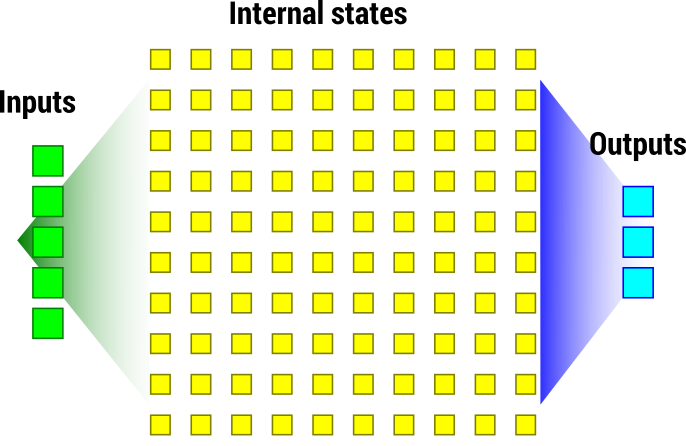
\includegraphics[width=0.7\textwidth]{Figures/simulation.png}
  \caption{Fan-out/fan-in structure of typical simulators used in hydrodynamics, solving the SWE over a grid \autocite{carbajal_emumore_2017}.}
  \label{fig:simulation}
\end{figure}

In contrast with simulators, emulators bridge the internal states: it goes from inputs to desired output directly, without passing through the internal states.
The emulator establishes a direct functional relationship between inputs and output.
It \emph{learns} this relationship from corresponding inputs-output sets.
Once the relationship is learned, and the model is validated, our emulator is ready to be exploited: it can now produce output predictions for new input values.
Fig.~\ref{fig:emulation} depicts this relationship bridging the internal states.

\begin{figure}[h]
  \centering
  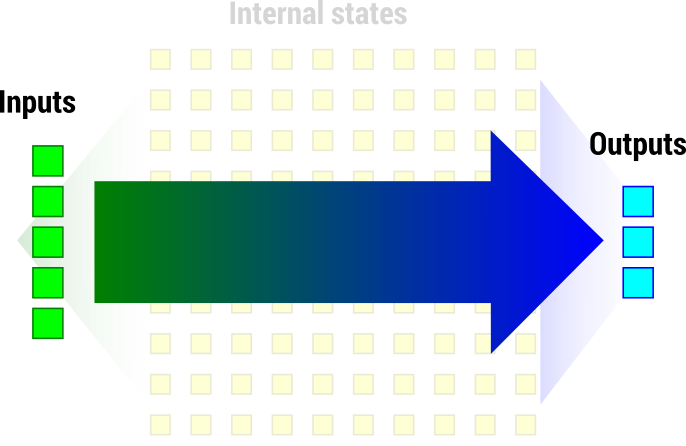
\includegraphics[width=0.7\textwidth]{Figures/emulation.png}
  \caption{Emulator functioning: a direct relationship linking the inputs to the outputs, independent from the internal states \autocite{carbajal_emumore_2017}.}
  \label{fig:emulation}
\end{figure}

The data needed for learning this relationship are inputs-output sets.
These are obtained by sampling the input space within the range needed with an appropriate technique, depending on the amount of input variables our problem has.
With every inputs-set a simulation is run and the desired output is extracted, generating this way our dataset.
The relationship has then to be learned with an appropriate technique: building an emulator is a regression problem, even more, it is an interpolation problem \autocite{carbajal_emumore_2017} which can be addressed with modern ML methods.\\

Emulators can mainly be divided into two groups: \emph{mechanistic} emulators and purely \emph{data-driven} emulators.
The first ones are built with methods able to encode prior knowledge of the system, introducing conditions guiding and constraining the interpolation problem.
The second ones, exploit techniques that blindly uncover relationships within the data, with no knowledge about the process generating them.
Whether to use a mechanistic or a purely data driven emulator is often quite subjective; studies try however to give guidelines helping with this choice \autocite{carbajal_appraisal_2016}.

\seb{ideal would be to introduce a workflow for implementing emulation}


% ------------------------------------------------------------------------------
\section{Regression and interpolation}
% ------------------------------------------------------------------------------

% * cite James et al., 2013 -> learning from data or predict outputs ->
%   GP -> can regress instead of interpolate, in order to establish easier
%   functional relationship

Key step when building an emulator is establishing the inputs-output relationship, namely solve the regression/interpolation problem.
For this many different methods exist; which one to choose may depend on the dimensions of the inputs space, the availability of data, the previous knowledge about the considered system, and weather we want to make predictions or learning functional relationships from our data.\\

Usually, when learning functional relationships from physical experimental data, we are trying to solve a regression problem.
The observation we are using are subject to errors assumed to be independent and Gaussian distributed due to the stochasticity of the problem.
Since the observation does not represent necessarily the true value, we then perform a regression, e.g. using the least squares (LS) method, minimizing the sum of squared residuals.
In this thesis, all of the experiments\footnote{Within the thesis, every reference to "experiment", if not differently stated, has to be read as "numerical experiment".} conducted are numerical experiments, namely simulations.
These are not subject to stochasticity.
Every simulation run with the same parameters produces the same output.
Since our emulator tries to reproduce the simulators behaviour, the observations should be rather interpolated than regressed.\\

Within this thesis four different types of regression/interpolation techniques, implemented within \citetalias{octave_community_gnu_2018} were used.

\begin{itemize}
\itemsep0em
  \item 1D-linear interpolation (\mintinline{octave}{interp1 (X, Y, XI, "linear")})
  \item 1D-cubic spline interpolation (\mintinline{octave}{interp1 (X, Y, XI, "spline")})
  \item 1D-linear regression (\mintinline{octave}{polyfit (X, Y, 1)})
  \item Gaussian Processes interpolation (package \citetalias{rasmussen_gaussian_2010})
\end{itemize}

From these, the GP interpolation is the most flexible and sophisticated one.
We can think of a GP as defining a distribution over functions.
A GP is fully specified by its \emph{mean} ($m(\bm{x})$) and \emph{covariance} function ($k(\bm{x},\bm{x}')$) \autocite{rasmussen_gaussian_2006}, which both may depend from hyperparameters.
The GP $f(\bm{x})$, with mean $m(\bm{x})$ and covariance $k(\bm{x},\bm{x}')$ is therefore a class of functions and is commonly written as:

\begin{equation}
  f(\bm{x}) \backsim \mathcal{GP}\left(m(\bm{x}), k(\bm{x},\bm{x}')\right)
\end{equation}

\noindent The hyperparameters define properties of this class of functions, like its smoothness for example.
When performing GP regression, we tune these hyperparameters in order to maximize the \emph{marginal likelihood} $p(\bm{y}\vert \bm{X})$, the probability of observing the output $\bm{y}$ given the inputs $\bm{X}$.
By tuning the hyperparameters we \seb{insert image Rasmussen p.20???} discriminate some classes of functions in favor of others, remaining at the end just with the "most probable class", with its mean (prediction) and its variance (confidence about the prediction).\seb{is this correct???}
If we require a smoothness which is higher than that of our data for example, the GP will not be able to interpolate the points anymore.
The result of the GP will therefore be the regression of the points.

By choosing specific mean and covariance functions, and setting constraints on the hyperparameters, GP allow us to encode prior knowledge in our model.


  
%mention GP can include priors
% we can enforce regression instead of interpolation













